%/*
% * SPDX-FileCopyrightText: 2021 Stefan Begerad <stefan@begerad.de>
% *
% * SPDX-License-Identifier: GPL-3.0-or-later
% */

%make document a Beamer presentaion
\documentclass{beamer}

%include preamble
%/*
% * SPDX-FileCopyrightText: 2021 Stefan Begerad <stefan@begerad.de>
% *
% * SPDX-License-Identifier: GPL-3.0-or-later
% */

%define outer theme (color and background)
%\usetheme{default}
%\usetheme{Goettingen}
%\usetheme{Darmstadt}
%\usetheme{Copenhagen}
\usetheme{Boadilla}
%\usetheme{Berlin}
%\usetheme{Berkeley}
%\usetheme{Bergen}
%\usetheme{Antibes}
%\usetheme{AnnArbor}
%\usetheme{Warsaw}
%\usetheme{Szeged}

%define color of theme
%\usecolortheme{default}
%\usecolortheme{beaver}
\usecolortheme{seahorse}

%add the following package to use links
%Define hyperref as last package, because it modifies other instructions!
\usepackage{hyperref}

\title[Dede]%optional
{Dede Echtzeit-Karte}

\subtitle{Offen, Unabhängig, Universell}

\author[Begerad]%(optional, for multiple authors)
{Stefan~Begerad}

\date[OTM, 6.2.2021]%(optional)
{Open Transport Meetup, June 2. 2021}

\logo{
\includegraphics[height=1cm]{dede/dedeLogo0128}}


\title[Dede]%optional
{Dede Echtzeit-Karte}

\subtitle{Offen, Unabhängig, Universell}

\author[Begerad]%(optional, for multiple authors)
{Stefan~Begerad}

\date[2022]%(optional)
{Vortrag, 2022}

%define the document
\begin{document}

%define title page
\begin{frame}
  \titlepage
\end{frame}

%outline table of content for the entire presentation
%use asterisk to indicate that this section shall not be part of the table
%the name of the section serves as the title of the slide
\AtBeginSection[]
{
    \begin{frame}
        \frametitle{Inhalt}
        \tableofcontents[currentsection]
    \end{frame}
}

\section{Dede Echtzeit-Karte}

%/*
% * SPDX-FileCopyrightText: 2021 Stefan Begerad <stefan@begerad.de>
% *
% * SPDX-License-Identifier: GPL-3.0-or-later
% */

%make document a Beamer presentaion
\documentclass{beamer}

%include preamble
%/*
% * SPDX-FileCopyrightText: 2021 Stefan Begerad <stefan@begerad.de>
% *
% * SPDX-License-Identifier: GPL-3.0-or-later
% */

%define outer theme (color and background)
%\usetheme{default}
%\usetheme{Goettingen}
%\usetheme{Darmstadt}
%\usetheme{Copenhagen}
\usetheme{Boadilla}
%\usetheme{Berlin}
%\usetheme{Berkeley}
%\usetheme{Bergen}
%\usetheme{Antibes}
%\usetheme{AnnArbor}
%\usetheme{Warsaw}
%\usetheme{Szeged}

%define color of theme
%\usecolortheme{default}
%\usecolortheme{beaver}
\usecolortheme{seahorse}

%add the following package to use links
%Define hyperref as last package, because it modifies other instructions!
\usepackage{hyperref}

\title[Dede]%optional
{Dede Echtzeit-Karte}

\subtitle{Offen, Unabhängig, Universell}

\author[Begerad]%(optional, for multiple authors)
{Stefan~Begerad}

\date[OTM, 6.2.2021]%(optional)
{Open Transport Meetup, June 2. 2021}

\logo{
\includegraphics[height=1cm]{dede/dedeLogo0128}}


%define the document
\begin{document}

%define title page
\begin{frame}
  \titlepage
\end{frame}

\section{Ueber Dede}

%/*
% * SPDX-FileCopyrightText: 2021 Stefan Begerad <stefan@begerad.de>
% *
% * SPDX-License-Identifier: GPL-3.0-or-later
% */

\begin{frame}{Merkmale}
  Dede: eine freie, unabhängige und universelle Echtzeit-Karte
  \begin{itemize}
  \item FREI: Gemeinschaftsprojejt als freie Software (wie in Redefreiheit und NICHT wie in Freibier;-)) veröffenlicht\footnote{\url{https://github.com/dancesWithCycles/dede-front-end}}
  \item UNABHÄNGIG: weder ausgerüstete Fahrzeugflotte noch eigene IT-Infrastuktur notwendig
  \item UNIVERSELL: beliebige Fahrzeuge wie Bahn, Bus, Car-Sharing, Fahrdienst, Straßenbahn, Tram, Taxi, usw. universell darstellt
  \end{itemize}
\end{frame}

\begin{frame}{Integration}
  Mobilitätsanbieter erscheinen auf der Dede Echtzeit-Karte, wenn Ihre Fahrer oder Betreiber die Bewegungsdaten selbstständig erzeugen. Dazu brauchen sie nicht mehr als ein konventionelles Smartphone mit Internet-Verbindung und die Dede App.
\end{frame}

\begin{frame}{Dede Echtzeit-Karte}
  %alternative alignment to center is left and right
  \begin{center}
    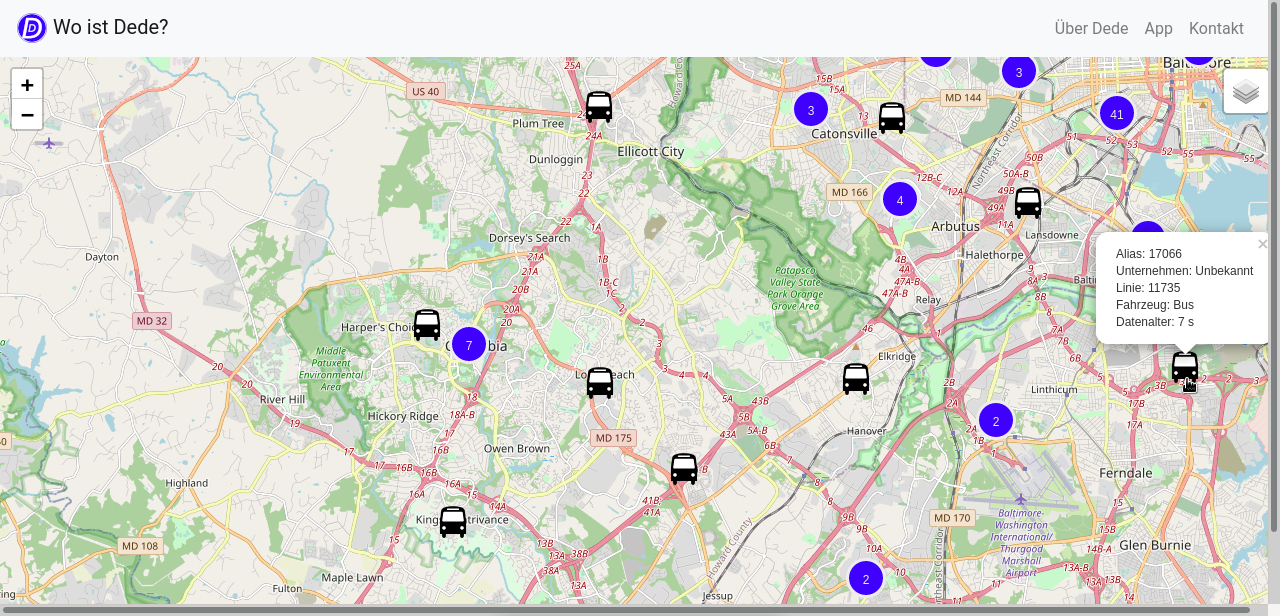
\includegraphics{dede/dede_real-time_map_crop}
  \end{center}
\end{frame}



%/*
% * SPDX-FileCopyrightText: 2021 Stefan Begerad <stefan@begerad.de>
% *
% * SPDX-License-Identifier: GPL-3.0-or-later
% */

\begin{frame}{Dede Konzept}
  %alternative alignment to center is left and right
  \begin{center}
    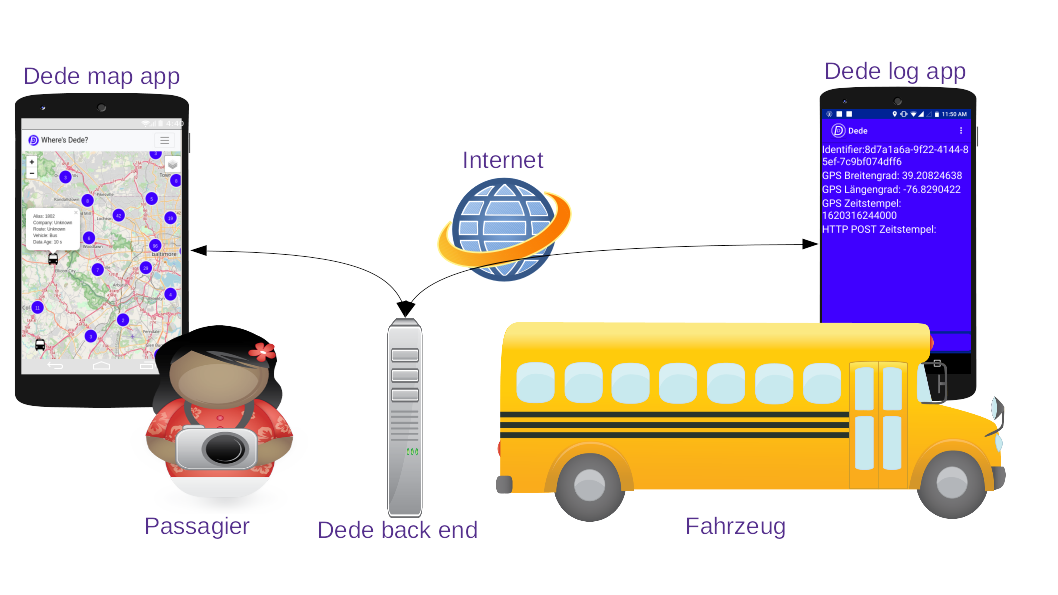
\includegraphics[width=\paperwidth]{dede/dede-concept}
  \end{center}
\end{frame}

\begin{frame}{Dede Konzept}
  Die Dede Echtzeit-Karte besteht aus drei Komponenten:
  \begin{itemize}
  \item Die Dede-App für Smartphones zeichnet die Bewegungsdaten des Fahrzeugs auf und überträgt sie per Internet an den Dede-Server.
  \item Der Dede-Server vermittelt zwischen Dede-App und Dede-Karte, so das die Karte NICHT jede App separat abfragen muss.
  \item Die Dede-Karte visualisiert die Bewegungdaten auf einer Karte in Echtzeit.
  \end{itemize}
\end{frame}


\end{document}


\end{document}
